% Created by tikzDevice version 0.12.6 on 2026-08-01 04:31:25
% !TEX encoding = UTF-8 Unicode
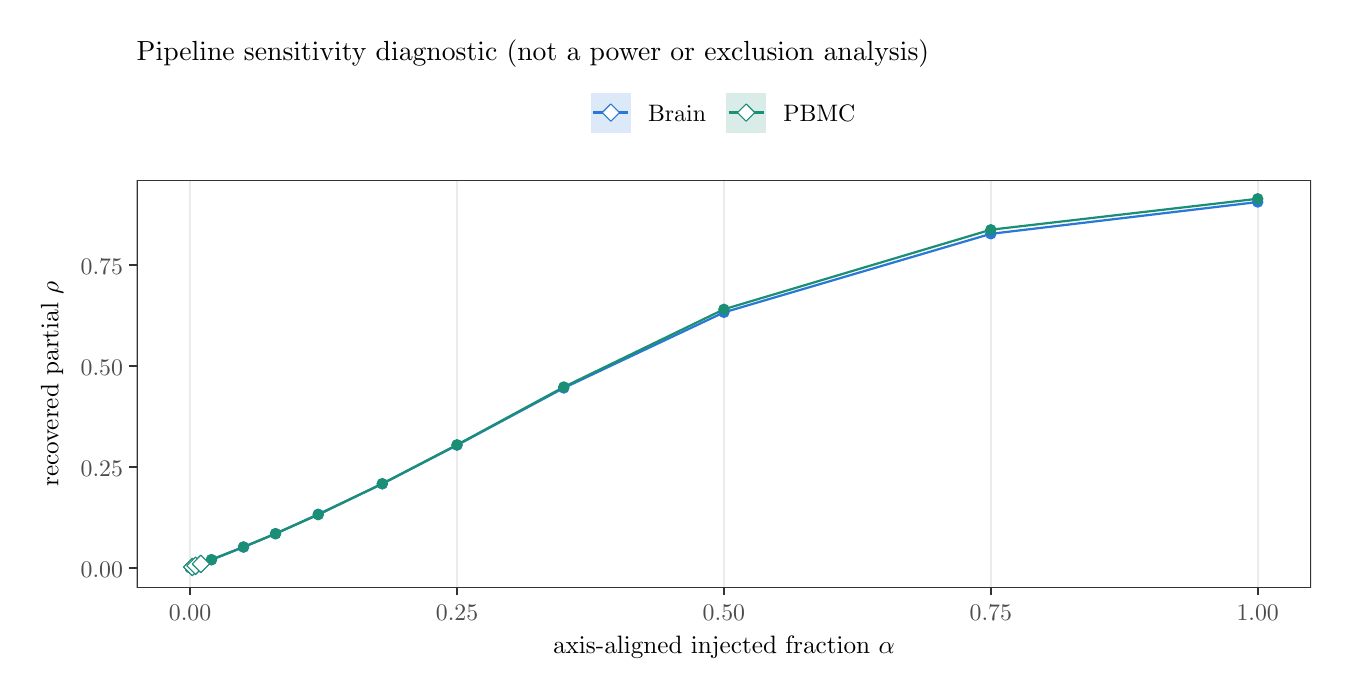
\begin{tikzpicture}[x=1pt,y=1pt]
\definecolor{fillColor}{RGB}{255,255,255}
\path[use as bounding box,fill=fillColor,fill opacity=0.00] (0,0) rectangle (469.75,231.26);
\begin{scope}
\path[clip] (  0.00,  0.00) rectangle (469.75,231.26);
\definecolor{drawColor}{RGB}{255,255,255}
\definecolor{fillColor}{RGB}{255,255,255}

\path[draw=drawColor,line width= 0.6pt,line join=round,line cap=round,fill=fillColor] (  0.00, -0.00) rectangle (469.76,231.26);
\end{scope}
\begin{scope}
\path[clip] ( 39.41, 28.85) rectangle (463.76,176.13);
\definecolor{fillColor}{RGB}{255,255,255}

\path[fill=fillColor] ( 39.41, 28.85) rectangle (463.75,176.13);
\definecolor{drawColor}{gray}{0.92}

\path[draw=drawColor,line width= 0.6pt,line join=round] ( 58.70, 28.85) --
	( 58.70,176.13);

\path[draw=drawColor,line width= 0.6pt,line join=round] (155.14, 28.85) --
	(155.14,176.13);

\path[draw=drawColor,line width= 0.6pt,line join=round] (251.58, 28.85) --
	(251.58,176.13);

\path[draw=drawColor,line width= 0.6pt,line join=round] (348.02, 28.85) --
	(348.02,176.13);

\path[draw=drawColor,line width= 0.6pt,line join=round] (444.47, 28.85) --
	(444.47,176.13);
\definecolor{fillColor}{RGB}{42,120,214}

\path[fill=fillColor,fill opacity=0.16] ( 58.70, 36.52) --
	( 66.41, 39.31) --
	( 77.99, 43.92) --
	( 89.56, 48.76) --
	(104.99, 55.93) --
	(128.14, 66.86) --
	(155.14, 80.71) --
	(193.72,101.33) --
	(251.58,128.58) --
	(348.02,156.80) --
	(444.47,168.25) --
	(444.47,168.25) --
	(348.02,156.72) --
	(251.58,128.27) --
	(193.72,100.80) --
	(155.14, 79.74) --
	(128.14, 66.07) --
	(104.99, 54.98) --
	( 89.56, 48.00) --
	( 77.99, 43.13) --
	( 66.41, 38.63) --
	( 58.70, 35.69) --
	cycle;

\path[] ( 58.70, 36.52) --
	( 66.41, 39.31) --
	( 77.99, 43.92) --
	( 89.56, 48.76) --
	(104.99, 55.93) --
	(128.14, 66.86) --
	(155.14, 80.71) --
	(193.72,101.33) --
	(251.58,128.58) --
	(348.02,156.80) --
	(444.47,168.25);

\path[] (444.47,168.25) --
	(348.02,156.72) --
	(251.58,128.27) --
	(193.72,100.80) --
	(155.14, 79.74) --
	(128.14, 66.07) --
	(104.99, 54.98) --
	( 89.56, 48.00) --
	( 77.99, 43.13) --
	( 66.41, 38.63) --
	( 58.70, 35.69);
\definecolor{fillColor}{RGB}{27,143,117}

\path[fill=fillColor,fill opacity=0.16] ( 58.70, 36.62) --
	( 66.41, 39.65) --
	( 77.99, 44.06) --
	( 89.56, 48.85) --
	(104.99, 55.55) --
	(128.14, 66.93) --
	(155.14, 80.82) --
	(193.72,101.77) --
	(251.58,129.55) --
	(348.02,158.28) --
	(444.47,169.43) --
	(444.47,169.43) --
	(348.02,158.22) --
	(251.58,129.39) --
	(193.72,101.08) --
	(155.14, 80.23) --
	(128.14, 66.12) --
	(104.99, 54.85) --
	( 89.56, 48.11) --
	( 77.99, 43.16) --
	( 66.41, 38.48) --
	( 58.70, 35.54) --
	cycle;

\path[] ( 58.70, 36.62) --
	( 66.41, 39.65) --
	( 77.99, 44.06) --
	( 89.56, 48.85) --
	(104.99, 55.55) --
	(128.14, 66.93) --
	(155.14, 80.82) --
	(193.72,101.77) --
	(251.58,129.55) --
	(348.02,158.28) --
	(444.47,169.43);

\path[] (444.47,169.43) --
	(348.02,158.22) --
	(251.58,129.39) --
	(193.72,101.08) --
	(155.14, 80.23) --
	(128.14, 66.12) --
	(104.99, 54.85) --
	( 89.56, 48.11) --
	( 77.99, 43.16) --
	( 66.41, 38.48) --
	( 58.70, 35.54);
\definecolor{drawColor}{RGB}{42,120,214}

\path[draw=drawColor,line width= 0.8pt,line join=round] ( 58.70, 36.07) --
	( 66.41, 38.99) --
	( 77.99, 43.57) --
	( 89.56, 48.38) --
	(104.99, 55.43) --
	(128.14, 66.42) --
	(155.14, 80.41) --
	(193.72,101.06) --
	(251.58,128.38) --
	(348.02,156.76) --
	(444.47,168.25);
\definecolor{drawColor}{RGB}{27,143,117}

\path[draw=drawColor,line width= 0.8pt,line join=round] ( 58.70, 36.17) --
	( 66.41, 39.01) --
	( 77.99, 43.61) --
	( 89.56, 48.43) --
	(104.99, 55.28) --
	(128.14, 66.48) --
	(155.14, 80.53) --
	(193.72,101.42) --
	(251.58,129.49) --
	(348.02,158.25) --
	(444.47,169.43);
\definecolor{drawColor}{RGB}{42,120,214}
\definecolor{fillColor}{RGB}{42,120,214}

\path[draw=drawColor,line width= 0.4pt,line join=round,line cap=round,fill=fillColor] ( 58.70, 36.07) circle (  1.86);

\path[draw=drawColor,line width= 0.4pt,line join=round,line cap=round,fill=fillColor] ( 66.41, 38.99) circle (  1.86);

\path[draw=drawColor,line width= 0.4pt,line join=round,line cap=round,fill=fillColor] ( 77.99, 43.57) circle (  1.86);

\path[draw=drawColor,line width= 0.4pt,line join=round,line cap=round,fill=fillColor] ( 89.56, 48.38) circle (  1.86);

\path[draw=drawColor,line width= 0.4pt,line join=round,line cap=round,fill=fillColor] (104.99, 55.43) circle (  1.86);

\path[draw=drawColor,line width= 0.4pt,line join=round,line cap=round,fill=fillColor] (128.14, 66.42) circle (  1.86);

\path[draw=drawColor,line width= 0.4pt,line join=round,line cap=round,fill=fillColor] (155.14, 80.41) circle (  1.86);

\path[draw=drawColor,line width= 0.4pt,line join=round,line cap=round,fill=fillColor] (193.72,101.06) circle (  1.86);

\path[draw=drawColor,line width= 0.4pt,line join=round,line cap=round,fill=fillColor] (251.58,128.38) circle (  1.86);

\path[draw=drawColor,line width= 0.4pt,line join=round,line cap=round,fill=fillColor] (348.02,156.76) circle (  1.86);

\path[draw=drawColor,line width= 0.4pt,line join=round,line cap=round,fill=fillColor] (444.47,168.25) circle (  1.86);
\definecolor{drawColor}{RGB}{27,143,117}
\definecolor{fillColor}{RGB}{27,143,117}

\path[draw=drawColor,line width= 0.4pt,line join=round,line cap=round,fill=fillColor] ( 58.70, 36.17) circle (  1.86);

\path[draw=drawColor,line width= 0.4pt,line join=round,line cap=round,fill=fillColor] ( 66.41, 39.01) circle (  1.86);

\path[draw=drawColor,line width= 0.4pt,line join=round,line cap=round,fill=fillColor] ( 77.99, 43.61) circle (  1.86);

\path[draw=drawColor,line width= 0.4pt,line join=round,line cap=round,fill=fillColor] ( 89.56, 48.43) circle (  1.86);

\path[draw=drawColor,line width= 0.4pt,line join=round,line cap=round,fill=fillColor] (104.99, 55.28) circle (  1.86);

\path[draw=drawColor,line width= 0.4pt,line join=round,line cap=round,fill=fillColor] (128.14, 66.48) circle (  1.86);

\path[draw=drawColor,line width= 0.4pt,line join=round,line cap=round,fill=fillColor] (155.14, 80.53) circle (  1.86);

\path[draw=drawColor,line width= 0.4pt,line join=round,line cap=round,fill=fillColor] (193.72,101.42) circle (  1.86);

\path[draw=drawColor,line width= 0.4pt,line join=round,line cap=round,fill=fillColor] (251.58,129.49) circle (  1.86);

\path[draw=drawColor,line width= 0.4pt,line join=round,line cap=round,fill=fillColor] (348.02,158.25) circle (  1.86);

\path[draw=drawColor,line width= 0.4pt,line join=round,line cap=round,fill=fillColor] (444.47,169.43) circle (  1.86);
\definecolor{drawColor}{RGB}{42,120,214}
\definecolor{fillColor}{RGB}{255,255,255}

\path[draw=drawColor,line width= 0.4pt,line join=round,line cap=round,fill=fillColor] ( 59.47, 33.25) --
	( 62.60, 36.38) --
	( 59.47, 39.51) --
	( 56.34, 36.38) --
	cycle;

\path[draw=drawColor,line width= 0.4pt,line join=round,line cap=round,fill=fillColor] ( 60.63, 33.60) --
	( 63.76, 36.73) --
	( 60.63, 39.86) --
	( 57.50, 36.73) --
	cycle;

\path[draw=drawColor,line width= 0.4pt,line join=round,line cap=round,fill=fillColor] ( 62.56, 34.39) --
	( 65.69, 37.52) --
	( 62.56, 40.65) --
	( 59.43, 37.52) --
	cycle;
\definecolor{drawColor}{RGB}{27,143,117}

\path[draw=drawColor,line width= 0.4pt,line join=round,line cap=round,fill=fillColor] ( 59.47, 33.23) --
	( 62.60, 36.36) --
	( 59.47, 39.49) --
	( 56.34, 36.36) --
	cycle;

\path[draw=drawColor,line width= 0.4pt,line join=round,line cap=round,fill=fillColor] ( 60.63, 33.70) --
	( 63.76, 36.83) --
	( 60.63, 39.96) --
	( 57.50, 36.83) --
	cycle;

\path[draw=drawColor,line width= 0.4pt,line join=round,line cap=round,fill=fillColor] ( 62.56, 34.36) --
	( 65.69, 37.49) --
	( 62.56, 40.62) --
	( 59.43, 37.49) --
	cycle;
\definecolor{drawColor}{gray}{0.20}

\path[draw=drawColor,line width= 0.6pt,line join=round,line cap=round] ( 39.41, 28.85) rectangle (463.75,176.13);
\end{scope}
\begin{scope}
\path[clip] (  0.00,  0.00) rectangle (469.75,231.26);
\definecolor{drawColor}{gray}{0.30}

\node[text=drawColor,anchor=base east,inner sep=0pt, outer sep=0pt, scale=  0.86] at ( 34.46, 32.72) {0.00};

\node[text=drawColor,anchor=base east,inner sep=0pt, outer sep=0pt, scale=  0.86] at ( 34.46, 69.22) {0.25};

\node[text=drawColor,anchor=base east,inner sep=0pt, outer sep=0pt, scale=  0.86] at ( 34.46,105.71) {0.50};

\node[text=drawColor,anchor=base east,inner sep=0pt, outer sep=0pt, scale=  0.86] at ( 34.46,142.21) {0.75};
\end{scope}
\begin{scope}
\path[clip] (  0.00,  0.00) rectangle (469.75,231.26);
\definecolor{drawColor}{gray}{0.20}

\path[draw=drawColor,line width= 0.6pt,line join=round] ( 36.66, 36.09) --
	( 39.41, 36.09);

\path[draw=drawColor,line width= 0.6pt,line join=round] ( 36.66, 72.59) --
	( 39.41, 72.59);

\path[draw=drawColor,line width= 0.6pt,line join=round] ( 36.66,109.08) --
	( 39.41,109.08);

\path[draw=drawColor,line width= 0.6pt,line join=round] ( 36.66,145.58) --
	( 39.41,145.58);
\end{scope}
\begin{scope}
\path[clip] (  0.00,  0.00) rectangle (469.75,231.26);
\definecolor{drawColor}{gray}{0.20}

\path[draw=drawColor,line width= 0.6pt,line join=round] ( 58.70, 26.10) --
	( 58.70, 28.85);

\path[draw=drawColor,line width= 0.6pt,line join=round] (155.14, 26.10) --
	(155.14, 28.85);

\path[draw=drawColor,line width= 0.6pt,line join=round] (251.58, 26.10) --
	(251.58, 28.85);

\path[draw=drawColor,line width= 0.6pt,line join=round] (348.02, 26.10) --
	(348.02, 28.85);

\path[draw=drawColor,line width= 0.6pt,line join=round] (444.47, 26.10) --
	(444.47, 28.85);
\end{scope}
\begin{scope}
\path[clip] (  0.00,  0.00) rectangle (469.75,231.26);
\definecolor{drawColor}{gray}{0.30}

\node[text=drawColor,anchor=base,inner sep=0pt, outer sep=0pt, scale=  0.86] at ( 58.70, 17.16) {0.00};

\node[text=drawColor,anchor=base,inner sep=0pt, outer sep=0pt, scale=  0.86] at (155.14, 17.16) {0.25};

\node[text=drawColor,anchor=base,inner sep=0pt, outer sep=0pt, scale=  0.86] at (251.58, 17.16) {0.50};

\node[text=drawColor,anchor=base,inner sep=0pt, outer sep=0pt, scale=  0.86] at (348.02, 17.16) {0.75};

\node[text=drawColor,anchor=base,inner sep=0pt, outer sep=0pt, scale=  0.86] at (444.47, 17.16) {1.00};
\end{scope}
\begin{scope}
\path[clip] (  0.00,  0.00) rectangle (469.75,231.26);
\definecolor{drawColor}{RGB}{0,0,0}

\node[text=drawColor,anchor=base,inner sep=0pt, outer sep=0pt, scale=  0.91] at (251.58,  5.21) {axis-aligned injected fraction $\alpha$};
\end{scope}
\begin{scope}
\path[clip] (  0.00,  0.00) rectangle (469.75,231.26);
\definecolor{drawColor}{RGB}{0,0,0}

\node[text=drawColor,rotate= 90.00,anchor=base,inner sep=0pt, outer sep=0pt, scale=  0.91] at ( 11.09,102.49) {recovered partial $\rho$};
\end{scope}
\begin{scope}
\path[clip] (  0.00,  0.00) rectangle (469.75,231.26);
\definecolor{fillColor}{RGB}{255,255,255}

\path[fill=fillColor] (197.28,187.13) rectangle (305.88,214.03);
\end{scope}
\begin{scope}
\path[clip] (  0.00,  0.00) rectangle (469.75,231.26);
\definecolor{fillColor}{RGB}{255,255,255}

\path[fill=fillColor] (202.78,192.63) rectangle (218.68,208.53);
\definecolor{fillColor}{RGB}{42,120,214}

\path[fill=fillColor,fill opacity=0.16] (203.50,193.34) rectangle (217.97,207.81);
\definecolor{drawColor}{RGB}{42,120,214}

\path[draw=drawColor,line width= 0.8pt,line join=round] (204.37,200.58) -- (217.09,200.58);
\definecolor{fillColor}{RGB}{42,120,214}

\path[draw=drawColor,line width= 0.4pt,line join=round,line cap=round,fill=fillColor] (210.73,200.58) circle (  1.86);
\definecolor{fillColor}{RGB}{255,255,255}

\path[draw=drawColor,line width= 0.4pt,line join=round,line cap=round,fill=fillColor] (210.73,197.45) --
	(213.86,200.58) --
	(210.73,203.71) --
	(207.60,200.58) --
	cycle;
\end{scope}
\begin{scope}
\path[clip] (  0.00,  0.00) rectangle (469.75,231.26);
\definecolor{fillColor}{RGB}{255,255,255}

\path[fill=fillColor] (251.66,192.63) rectangle (267.56,208.53);
\definecolor{fillColor}{RGB}{27,143,117}

\path[fill=fillColor,fill opacity=0.16] (252.37,193.34) rectangle (266.85,207.81);
\definecolor{drawColor}{RGB}{27,143,117}

\path[draw=drawColor,line width= 0.8pt,line join=round] (253.25,200.58) -- (265.97,200.58);
\definecolor{fillColor}{RGB}{27,143,117}

\path[draw=drawColor,line width= 0.4pt,line join=round,line cap=round,fill=fillColor] (259.61,200.58) circle (  1.86);
\definecolor{fillColor}{RGB}{255,255,255}

\path[draw=drawColor,line width= 0.4pt,line join=round,line cap=round,fill=fillColor] (259.61,197.45) --
	(262.74,200.58) --
	(259.61,203.71) --
	(256.48,200.58) --
	cycle;
\end{scope}
\begin{scope}
\path[clip] (  0.00,  0.00) rectangle (469.75,231.26);
\definecolor{drawColor}{RGB}{0,0,0}

\node[text=drawColor,anchor=base west,inner sep=0pt, outer sep=0pt, scale=  0.86] at (224.18,197.21) {Brain};
\end{scope}
\begin{scope}
\path[clip] (  0.00,  0.00) rectangle (469.75,231.26);
\definecolor{drawColor}{RGB}{0,0,0}

\node[text=drawColor,anchor=base west,inner sep=0pt, outer sep=0pt, scale=  0.86] at (273.06,197.21) {PBMC};
\end{scope}
\begin{scope}
\path[clip] (  0.00,  0.00) rectangle (469.75,231.26);
\definecolor{drawColor}{RGB}{0,0,0}

\node[text=drawColor,anchor=base west,inner sep=0pt, outer sep=0pt, scale=  1.00] at ( 39.41,219.46) {Pipeline sensitivity diagnostic (not a power or exclusion analysis)};
\end{scope}
\end{tikzpicture}
